\documentclass[handout]{beamer} % Use the beamer class for presentations, 'handout' option to suppress \pause

\input{Lecture-Slides/preamble.txt}

% Define the transition slide command
\newcommand{\transitionslide}[1]{
    \begin{frame}[plain]
        \centering
        \vspace{1cm}
        \Huge
        \textcolor{moonstoneblue!150}{\textbf{#1}}
    \end{frame}
}

% Packages for math and plots
\usepackage{amsmath}
\usepackage{graphicx}
\usepackage{booktabs}

\usepackage{pgfplots}

% Nice color sets, see see http://colorbrewer2.org/
\usepgfplotslibrary{colorbrewer}
% initialize Set1-4 from colorbrewer (we're comparing 4 classes),
\pgfplotsset{compat = 1.18, cycle list/Set1-8}
% Tikz is loaded automatically by pgfplots
\usetikzlibrary{pgfplots.statistics, pgfplots.colorbrewer}

% provides \pgfplotstabletranspose
\usepackage{pgfplotstable}
\usepackage{filecontents}


% Title and author information
\title{Introduction to Statistical Methods in Political Science}
\subtitle{Lecture 8: Statistical Inference for One Proportion}
\author{Ignacio Urbina \texorpdfstring{\\ \vspace{0.3em}}{ } \scriptsize \textcolor{gray}{Ph.D. Candidate in Political Science}}
\date{}

\begin{document}

% Slide 1: Title Slide
\begin{frame}
    \titlepage
\end{frame}

% Slide 2: Learning Objectives
\begin{frame}{Learning Objectives}
    \begin{itemize}
        \item \textbf{Understand:}
        \begin{itemize}
            \item Confidence Intervals for \( p \)
            \item Hypothesis Testing for \( p \)
        \end{itemize}
    \end{itemize}
\end{frame}

\section{Sample Proportion - Sampling Distribution}
\transitionslide{Sample Proportion - Sampling Distribution}

% Slide 3: Proportions
\begin{frame}{Inference with Proportions}
    \begin{itemize}
        \item \textbf{Key Terms:}
        \begin{itemize}
            \item \textbf{Population Proportion (\( p \))}:
            \[
                p = \frac{\text{Number of successes in population}}{\text{Total population size}} = \frac{S}{N}
            \]
            \item \textbf{Sample Proportion (\( \hat{p} \))}:
            \[
                \hat{p} = \frac{S_n}{n}
            \]
            \[
               S_n= \text{Number of successes in the sample}, \quad n = \text{Sample size}
            \]
        \end{itemize}
        \item \textbf{Purpose:} Infer \( p \) from \( \hat{p} \)
    \end{itemize}
\end{frame}

\begin{frame}{Intuition Behind Inference}
    \begin{itemize}
        \item \textbf{Concept:} Statistical inference involves estimating an unknown population parameter based on sample data.
        \item \textbf{Sample Variability:} Measuring the same quantity multiple times with slight variations each time.

    \[
        \text{Repeated sampling} \Rightarrow \hat{p}_1, \hat{p}_2, \ldots, \hat{p}_k
    \]
    \item \textbf{Example}: Assume you collect data from a sample of size $n$, and you compute the proportion of people vaccinated against some virus, $\hat{p}$.
    \end{itemize}
\end{frame}

% Slide 5: Visual for Presenting and Describing the Problem
\begin{frame}{Visualizing Sample Variability in Vaccination Rates}
    \begin{figure}
        \centering
        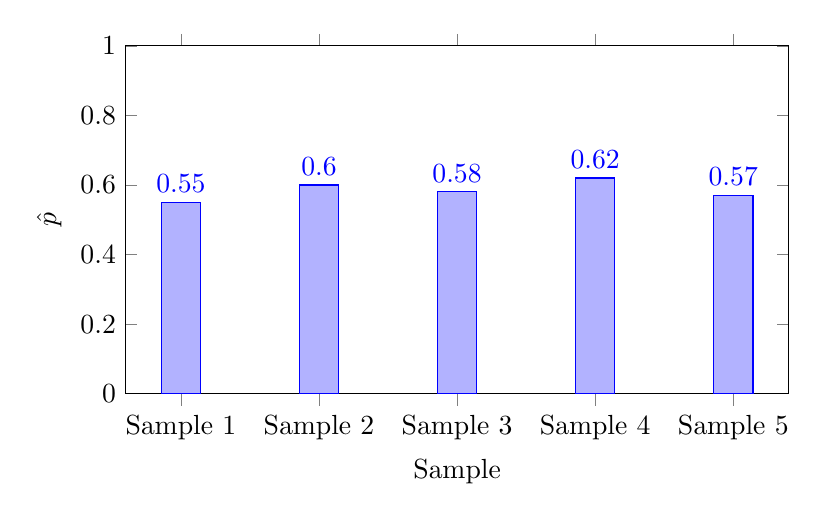
\begin{tikzpicture}
            \begin{axis}[
                ybar,
                symbolic x coords={Sample 1, Sample 2, Sample 3, Sample 4, Sample 5},
                xtick=data,
                ymin=0, ymax=1,
                ylabel={\( \hat{p} \)},
                xlabel={Sample},
                width=10cm,
                height=6cm,
                bar width=0.5cm,
                nodes near coords,
                nodes near coords align={vertical},
            ]
                \addplot coordinates {
                    (Sample 1,0.55) (Sample 2,0.60) (Sample 3,0.58) (Sample 4,0.62) (Sample 5,0.57)
                };
            \end{axis}
        \end{tikzpicture}
        \caption{Variability in Sample Proportions (\( \hat{p} \))}
    \end{figure}
\end{frame}

\begin{frame}{Sample Proportion}
Let:
\[ \{ X_i\}_{i=1}^{N} \text{ be a sample collected via simple random sampling}\]
\[
X_1, X_2, \dots, X_n \sim \text{Bernoulli}(p)
\]
\[
\hat{p} = \frac{1}{n} \sum_{i=1}^n X_i
\]
Note that any $X_k$ and $X_j$:
\begin{itemize}
    \item Are identically distributed. So, $E[X_k]=E[X_j]=p$, and $V[X_k]=V[X_j]=p(1-p)$.
    \item Are independent. So, this implies the following variance of a linear combination of two values, $V((X_k + X_j)/2) = (1/4)\cdot V(X_k+X_j) = (1/4)\cdot [p(1-p) + p(1-p)] = \frac{p(1-p)}{2}$

\end{itemize}
\end{frame}

\begin{frame}{Expectation and Variance}

Population mean:
\[
\mathbb{E}[\hat{p}]
= \mathbb{E}\left[\frac{1}{n} \sum_{i=1}^n X_i\right]
= \frac{1}{n} \sum_{i=1}^n \mathbb{E}[X_i]
= p
\]
Variance:
\[
\text{Var}(\hat{p})
= \text{Var}\left(\frac{1}{n} \sum_{i=1}^n X_i\right)
= \frac{1}{n^2} \sum_{i=1}^n \text{Var}(X_i)
\]
\[
= \frac{1}{n^2} \cdot n \cdot p(1 - p)
= \frac{p(1 - p)}{n}
\]
\end{frame}

% Slide 8: Motivation for Inference: Sample Variability
\begin{frame}{Sample Variability and Sampling Distribution}
    \begin{itemize}
        \item \textbf{Repeated Sampling:} Each sample yields a different \( \hat{p} \).
        \item \textbf{Objective:} Quantify the variability of \( \hat{p} \).
    \[
        \text{Variance of } \hat{p} = \frac{p(1 - p)}{n}
    \]
    \[
        \text{Standard Error (SE)} = \sqrt{\frac{p(1 - p)}{n}}
    \]
     \item \textbf{Sampling Distribution:} If the sample size is large, we can use the CLT to approximate the sampling distribution of $\hat{p}$:
    \[
        \hat{p} \approx N\left(p, \frac{p(1-p)}{n}\right)
    \]
    \end{itemize}
\end{frame}

\section{Confidence Intervals}
\transitionslide{Confidence Intervals}

% Slide 1: Introduction to Confidence Intervals
\begin{frame}
    \frametitle{What is a Confidence Interval?}
    \begin{itemize}
        \item A confidence interval (CI) provides a range of values within which we are fairly certain the true population parameter (e.g., a proportion or mean) lies.
        \item CIs give us an idea of how reliable our estimate is, based on our sample data.
        \item They quantify the uncertainty around our estimate, offering a range likely to contain the true value.
    \end{itemize}
\end{frame}

% Slide 3: Confidence Interval Formula
\begin{frame}
    \frametitle{Confidence Interval Formula}
    \begin{itemize}
        \item For an unknown population proportion \( p \), in large samples the sample proportion \( \hat{p} = \frac{S_n}{n} \) is approximately normally distributed:
    \end{itemize}
    \[
    \frac{\hat{p} - p}{\sqrt{\frac{p(1-p)}{n}}} \approx Z \sim N(0,1)
    \]
    \begin{itemize}
        \item To calculate a 95\% confidence interval, we utilize:
    \end{itemize}
    \[
    P(-1.96 \leq Z \leq 1.96) = 0.95
    \]
\end{frame}


% Slide 5: Confidence Interval Range
\begin{frame}
    \frametitle{Calculating the Confidence Interval Range}
    \begin{itemize}
        \item Translating the standardization back to our interval:
    \end{itemize}
    \[
    P(-1.96 \leq Z \leq 1.96) = 0.95
    \]
    \[
    P(-1.96 \leq  \frac{\hat{p} - p}{\sqrt{\frac{p(1-p)}{n}}} \leq 1.96) \approx 0.95
    \]
    \[
    P\left(\hat{p} - 1.96\sqrt{\frac{p(1-p)}{n}} \leq p \leq \hat{p} + 1.96\sqrt{\frac{p(1-p)}{n}}\right) \approx 0.95
    \]
    \begin{itemize}
        \item We are 95\% confident that the true population parameter \( p \) lies within this calculated interval.
    \end{itemize}
\end{frame}

% Slide 4: Interpretation of the Formula
\begin{frame}
    \frametitle{Logic Behind the Confidence Interval Derivation}
    \begin{itemize}
        \item We start by making a reasonable assumption about the sampling distribution for $\hat{p}$.
        \item Then we standardize $\hat{p}$ into a $Z$-score, and estimate the variability due to sampling using the standard normal.
        \item When we say \( P(-1.96 \leq Z \leq 1.96) = 0.95 \), we mean that 95\% of possible outcomes will fall within this $\pm1.96$ range under the normal distribution.
        \item Then, by using the properties of the normal distribution, we define a range within which the true proportion \( p \) likely lies.
    \end{itemize}
\end{frame}

\begin{frame}
    \frametitle{The Anatomy of a Confidence Interval}
    \begin{itemize}
        \item Is a procedure that depends on realized values for a random variables, in this case, $\hat{p}$.
        \item Thus, it is subject to sample variability.
        \item Note that for each given confidence interval, either the true proportion is or isn't contained. The true proportion is a fixed quantity.
        \item We ask, what percentage of the time will the confidence interval capture the true proportion? That is the confidence level, or one minus alpha ($1-\alpha$). Alpha is the significance level.
        \item Over the long run (note this thought exercise is informed by the sampling distribution of $\hat{p}$), we expect that $p$ will be included $(1-\alpha)$\% of the time.
    \end{itemize}
\end{frame}

% Slide 2: Confidence Interval Intuition
\begin{frame}
    \frametitle{Intuition Behind Confidence Intervals}
    \begin{quote}
        Were this procedure to be repeated on numerous samples, the fraction of calculated confidence intervals (which would differ for each sample) that encompass the true population parameter would tend toward 95\%.
    \end{quote}
\end{frame}



% Slide 6: Estimating the Standard Error
\begin{frame}
    \frametitle{Estimating the Standard Error (SE)}
    \begin{itemize}
        \item The standard error for the proportion is given by:
        \[
        \text{SE} = \sqrt{\frac{p(1-p)}{n}}
        \]
        \item Since \( p \) is unknown, by the plugin principle, we use the sample proportion \( \hat{p} \) to estimate it:
        \[
        \text{SE} \approx \sqrt{\frac{\hat{p}(1-\hat{p})}{n}}
        \]
    \end{itemize}
\end{frame}

% Slide 7: Calculating the Margin of Error (MOE)
\begin{frame}
    \frametitle{Margin of Error (MOE)}
    \begin{itemize}
        \item The margin of error (MOE) is a statistic expressing the amount of random sampling error in the results of a survey.
        \item The margin of error is found by multiplying the SE by the critical value (1.96 for a 95\% confidence level):
        \[
            \text{MOE} = 1.96 \times \text{SE}(\hat{p})
        \]
        \item For a general confidence interval level of $(1-\alpha)$:
        \[
            \text{MOE} = z_{1-\frac{\alpha}{2}} \times \text{SE}(\hat{p})
        \]
        where $z_{1-\frac{\alpha}{2}}$ is the critical value from the standard normal distribution.
    \end{itemize}
\end{frame}


% Slide 8: Constructing the Confidence Interval
\begin{frame}
    \frametitle{Constructing the Confidence Interval}
    \begin{itemize}
        \item Finally, the confidence interval is given by:
    \[
    \left[\hat{p} - \text{MOE}, \, \hat{p} + \text{MOE}\right]
    \]
    \item For a 95\% CI:
       \[
    \text{MOE} = 1.96 \times \text{SE}(\hat{p}) = 1.96 \times \sqrt{\frac{\hat{p}(1-\hat{p})}{n}}
    \]
        \item This interval provides an estimated range that, with 95\% confidence, contains the true population proportion \( p \).
    \end{itemize}
\end{frame}

% Slide: General Formula for Confidence Intervals
\begin{frame}
    \frametitle{General Formula for Confidence Intervals for $p$}
    \begin{itemize}
        \item Invoking the CLT:
        \[
        \hat{p} \sim N\left(p, \frac{p(1-p)}{n}\right)
        \]
        \item Thus, the Z-score standardized form:
        \[
        Z = \frac{\hat{p} - p}{\sqrt{\frac{p(1-p)}{n}}} \sim N\left( 0, 1 \right)
        \]
        \item To construct a confidence interval with confidence level \( 1 - \alpha \), we use the critical value \( z_{1-\alpha/2} \) such that:
        \[
        P\left(Z < z_{1-\alpha/2}\right) = 1 - \frac{\alpha}{2}
        \]
        \item The general confidence interval for \( p \) becomes:
        \[
        \hat{p} \pm z_{1-\alpha/2} \cdot \sqrt{\frac{\hat{p}(1 - \hat{p})}{n}}
        \]
    \end{itemize}
\end{frame}


\begin{frame}
    \frametitle{Steps to Calculate a 99\% Confidence Interval}
    \begin{enumerate}
        \item \textbf{Determine the Confidence Level and Critical Value:}
        \begin{itemize}
            \item For a 99\% confidence interval, the critical value from the normal distribution is approximately \( Z = 2.576 \).
        \end{itemize}

        \item \textbf{Estimate the Standard Error (SE):}
        \begin{itemize}
            \item Use the sample proportion \( \hat{p} \) to estimate \( SE \):
            \[
            \text{SE} \approx \sqrt{\frac{\hat{p}(1 - \hat{p})}{n}}
            \]
        \end{itemize}

        \item \textbf{Calculate the Margin of Error (MOE):}
        \begin{itemize}
            \item Multiply the SE by the critical value:
            \[
            \text{MOE} = 2.576 \times \text{SE}
            \]
        \end{itemize}

        \item \textbf{Construct the Confidence Interval:}
        \begin{itemize}
            \item Add and subtract the MOE from the sample proportion \( \hat{p} \):
            \[
            \left[ \hat{p} - \text{MOE}, \, \hat{p} + \text{MOE} \right]
            \]
            \item This interval provides a 99\% confidence range for the true population proportion \( p \).
        \end{itemize}
    \end{enumerate}
\end{frame}
% Slide X: Example - Confidence Interval Calculation for 95% and 99%
\begin{frame}{Applied Example: Computing 95\% and 99\% Confidence Intervals}
    \textbf{Problem Statement:}
    \begin{itemize}
        \item A public health survey finds that out of a sample of 400 people, 120 are vaccinated.
        \item We wish to calculate the 95\% and 99\% confidence intervals for the true proportion of vaccinated individuals in the population.
    \end{itemize}

    \textbf{Given Data:}
    \begin{itemize}
        \item Sample size (\( n \)) = 400
        \item Sample proportion (\( \hat{p} \)) = \(\frac{120}{400} = 0.300\)
    \end{itemize}
\end{frame}

% Slide X+1: Step 1 - Calculate Standard Error (SE)
\begin{frame}{Step 1: Calculate Standard Error (SE)}
    \begin{itemize}
        \item \textbf{Formula:} \( \text{SE} = \sqrt{\frac{\hat{p}(1 - \hat{p})}{n}} \)
        \item \textbf{Calculation:}
\begin{align*}
    \text{SE} = \sqrt{\frac{0.300 \times (1 - 0.300)}{400}} = \sqrt{\frac{0.300 \times 0.700}{400}} &= \sqrt{\frac{0.210}{400}}  \\
                                                                                                    &= \sqrt{0.000525} \\
                                                                                                    &\approx 0.023
\end{align*}


    \end{itemize}
\end{frame}

% Slide X+2: Step 2 - Calculate 95% Confidence Interval
\begin{frame}{Step 2: Calculate 95\% Confidence Interval}
    \begin{itemize}
        \item \textbf{Critical Value:} For a 95\% confidence level, \( Z_{1-0.05/2} = Z_{0.975}  = 1.96 \)
        \item \textbf{Margin of Error (MOE):}
        \[
            \text{MOE} = 1.96 \times \text{SE} = 1.96 \times 0.023 \approx 0.045
        \]
        \item \textbf{95\% CI Calculation:}
        \[
            \text{CI} = \hat{p} \pm \text{MOE} = 0.300 \pm 0.045
        \]
        \[
            \text{95\% CI} = [0.255, 0.345]
        \]
    \end{itemize}
\end{frame}

% Slide X+3: Step 3 - Calculate 99% Confidence Interval
\begin{frame}{Step 3: Calculate 99\% Confidence Interval}
    \begin{itemize}
        \item \textbf{Critical Value:} For a 99\% confidence level (i.e., $\alpha=0.01$), \( Z_{1-0.01/2} = Z_{0.995} = 2.576 \)
        \item \textbf{Margin of Error (MOE):}
        \[
            \text{MOE} = 2.576 \times \text{SE} = 2.576 \times 0.023 \approx 0.059
        \]
        \item \textbf{99\% CI Calculation:}
        \[
            \text{CI} = \hat{p} \pm \text{MOE} = 0.300 \pm 0.059
        \]
        \[
            \text{99\% CI} = [0.241, 0.359]
        \]
    \end{itemize}
\end{frame}

% Slide X+4: Interpretation of 95% and 99% Confidence Intervals
\begin{frame}{Interpretation of 95\% and 99\% Confidence Intervals}
    \begin{itemize}
        \item \textbf{95\% CI (0.255, 0.345):}
        \begin{itemize}
            \item We are 95\% confident that the true proportion of vaccinated individuals is between 25.5\% and 34.5\%.
        \end{itemize}
        \item \textbf{99\% CI (0.241, 0.359):}
        \begin{itemize}
            \item We are 99\% confident that the true proportion of vaccinated individuals is between 24.1\% and 35.9\%.
        \end{itemize}
        \item \textbf{Observations:}
        \begin{itemize}
            \item The 99\% CI is wider than the 95\% CI, reflecting greater confidence and a broader range for the estimate.
        \end{itemize}
    \end{itemize}
\end{frame}

\begin{frame}
\frametitle{Which Percent of Future Sample Proportions Will Fall in Our CI?}
\begin{itemize}
    \item A 95\% confidence interval captures the \textbf{true parameter} \( p \) in 95\% of repeated samples.
    \item But the interval is built around one observed sample proportion \( \hat{p}_{\text{orig}} \).
    \item \textbf{Future sample proportions} \( \hat{p}_{\text{new}} \) follow a distribution centered at \( p \), not at \( \hat{p}_{\text{orig}} \).
    \item Therefore, the long-run probability that future \( \hat{p}_{\text{new}} \) falls within the \textbf{fixed CI} from the past will be most likely lower than 95\%.
\end{itemize}
But note this is a \textbf{moot question}. We really care about $p$, not $\hat{p}$!
\end{frame}


\section{Hypothesis Testing}
\transitionslide{Hypothesis Testing}

% Slide X+5: Introduction to Hypothesis Testing
\begin{frame}{Introduction to Hypothesis Testing}
    \begin{itemize}
        \item \textbf{Why Test Hypotheses?}
        \begin{itemize}
            \item Often, we want to know if a certain belief or assumption about a population is likely to be true based on our sample data.
            \item For example, we might wonder, “Is the vaccination rate really 30\% in the general population, or is it different?”
        \end{itemize}

        \item \textbf{Hypothesis Testing:} A systematic way to check if our data supports or refutes our initial belief.
        \begin{itemize}
            \item Imagine having a statement about a population—our hypothesis—and then using data to evaluate if there’s enough evidence to challenge that statement.
        \end{itemize}
    \end{itemize}
\end{frame}

% Slide X+6: Hypothesis Testing Approach
\begin{frame}{How Hypothesis Testing Works}
    \begin{itemize}
        \item \textbf{Formulating Two Opposing Claims:}
        \begin{itemize}
            \item We start with two possible claims about a population measure, such as a proportion.
            \item One claim (the \textit{null hypothesis}) represents a baseline assumption, often suggesting "no change" or "no effect."
            \item The other claim (the \textit{alternative hypothesis}) suggests there’s a meaningful difference from the null.
        \end{itemize}

        \item \textbf{Gathering Evidence:}
        \begin{itemize}
            \item Using sample data, we evaluate if there’s enough evidence to support or refute our baseline assumption.
            \item Just as in a courtroom, we start with a presumption (the null hypothesis is true) and only reject it if the evidence is strong.
        \end{itemize}

        \item \textbf{Making a Decision:}
        \begin{itemize}
            \item If our sample data aligns well with the null hypothesis, we “fail to reject” it.
            \item If the data strongly contradicts the null hypothesis, we “reject” it in favor of the alternative hypothesis.
        \end{itemize}
    \end{itemize}
\end{frame}

% Slide X+7: Introducing the Test Statistic for Proportions
\begin{frame}{Introducing the Test Statistic}
    \begin{itemize}
        \item \textbf{What is a Test Statistic?}
        \begin{itemize}
            \item A test statistic is a number we calculate from our sample data to help us decide if our sample provides enough evidence to challenge the null hypothesis.
            \item Think of it as a “score” that tells us how far our sample result is from what we would expect if the null hypothesis were true.
        \end{itemize}

        \item \textbf{The Formula for the Test Statistic (for Proportions):}
\[
        Z = \frac{\hat{p} - p_0}{\sqrt{\frac{p_0(1 - p_0)}{n}}}
\]

        \item \textbf{Defining Each Term:}
        \begin{itemize}
            \item $\hat{p}$: The \textbf{sample proportion}.
            \item $p_0$: The \textbf{null hypothesized proportion}, or the value of the proportion we are assuming is true under the null hypothesis.
            \item $n$: The \textbf{sample size}, or the number of individuals in our sample.
            \item $\sqrt{\frac{p_0(1 - p_0)}{n}} $: The \textbf{standard error (SE)} of $\hat{p}$ assuming the null hypothesis.
        \end{itemize}
    \end{itemize}
\end{frame}

% Slide X+8: Intuition Behind the Test Statistic and its Interpretation
\begin{frame}{Understanding the Test Statistic and its Interpretation}
    \begin{itemize}
        \item \textbf{What Units Does the Test Statistic Use?}
        \begin{itemize}
            \item The test statistic $Z$ is measured in \textbf{standard error units}.
            \item It represents how many standard errors the sample proportion $\hat{p} $ is away from the null hypothesis proportion $p_0$.
        \end{itemize}

        \item \textbf{Why Large Absolute Values of $Z$ Suggest Evidence Against the Null:}
        \begin{itemize}
            \item If $Z$ is large (either positive or negative), it means $\hat{p}$ is far from $p_0$ in terms of \emph{expected variability under the assumption of the null hypothesis}, which may indicate that the null hypothesis is unlikely.
        \end{itemize}
    \end{itemize}
\end{frame}

% Slide X+9: Formal Setup of a Hypothesis Test
\begin{frame}{Formal Setup of a Hypothesis Test}
    \begin{itemize}
        \item \textbf{Defining Hypotheses:}
        \begin{itemize}
            \item We write the \textbf{null hypothesis} as: \( H_0: p = p_0 \)
            \item The \textbf{alternative hypothesis} represents what we want to test against \( H_0 \). For example:
            \begin{itemize}
                \item \( H_a: p \neq p_0 \) (two-tailed)
                \item \( H_a: p > p_0 \) (one-tailed, right)
                \item \( H_a: p < p_0 \) (one-tailed, left)
            \end{itemize}
        \end{itemize}

        \item \textbf{Significance Level (\( \alpha \)):}
        \begin{itemize}
            \item \( \alpha \) is the threshold probability for deciding when to reject \( H_0 \).
            \item Common values for \( \alpha \) are 0.05 or 0.01, indicating a 5% or 1% risk of rejecting \( H_0 \) when it is actually true.
            \item If the probability of observing our test statistic (or more extreme) under \( H_0 \) is less than \( \alpha \), we reject \( H_0 \).
            \item \( \alpha \) is a standard, carefully chosen rule that guides us on when to be confident enough to reject \( H_0 \) based on how unlikely our observed data is under the null hypothesis.
        \end{itemize}
    \end{itemize}
\end{frame}

% Slide X+10: Intuition of the Significance Level
\begin{frame}{Intuition of the Significance Level}
    \begin{itemize}
        \item \textbf{Understanding \( \alpha \) as a Tolerance for Error:}
        \begin{itemize}
            \item The significance level \( \alpha \) defines how much evidence we need to reject \( H_0 \).
            \item It represents our tolerance for being wrong—a boundary for the probability of making a Type I error (rejecting \( H_0 \) when it’s actually true).
            \item Typical values (e.g., \( \alpha = 0.05 \)) mean we accept up to a 5\% risk of mistakenly rejecting \( H_0 \).
        \end{itemize}

        \item \textbf{The Rejection Region:}
        \begin{itemize}
            \item The rejection region is determined by \( \alpha \) and lies at the "extreme ends" of the distribution under \( H_0 \).
            \item If our test statistic falls in this region, it suggests that our observed result is too rare under \( H_0 \) for us to retain it with confidence.
            \item Thus, if our result is in the rejection region, we are willing to reject \( H_0 \) because it fits our set threshold for "unusual" results.
        \end{itemize}


    \end{itemize}
\end{frame}

% Slide X+10: Example Setup - Hypothesis Test for Voting Preference
\begin{frame}{Example: Hypothesis Test for Voting Preference}
    \begin{itemize}
        \item \textbf{Context:} Pew Research surveyed 1,000 participants on voting preference.
        \begin{itemize}
            \item 52\% of the sample say they will vote for Trump.
            \item We want to test if the true proportion who will vote for Harris is 51\% (i.e., the true proportion of Trump voters is 49\%).
        \end{itemize}

        \item \textbf{Hypotheses:}
        \begin{itemize}
            \item Null hypothesis \( H_0: p = 0.49 \)
            \item Alternative hypothesis \( H_a: p \neq 0.49 \) (two-tailed test)
        \end{itemize}

        \item \textbf{Significance Level:} Set \( \alpha = 0.05 \)
    \end{itemize}
\end{frame}

% Slide X+11: Solution - Calculating the Test Statistic and Conclusion
\begin{frame}{Solution: Test Statistic and Conclusion}
    \begin{itemize}
        \item \textbf{Sample Proportion:} \( \hat{p} = 0.52 \)

        \item \textbf{Standard Error (SE):}
\[
        \text{SE} = \sqrt{\frac{p_0(1 - p_0)}{n}} = \sqrt{\frac{0.49 \times (1 - 0.49)}{1000}} \approx 0.0158
\]

        \item \textbf{Test Statistic:}
\[
        Z = \frac{\hat{p} - p_0}{\text{SE}} = \frac{0.52 - 0.49}{0.0158} \approx 1.898
\]

        \item \textbf{Decision:}
        \begin{itemize}
            \item Since \( Z = 1.898 \) is within the range of \( [-1.96, 1.96] \), we \textbf{fail to reject} \( H_0 \) at \( \alpha = 0.05 \).
            \item Conclusion: There is not enough evidence to suggest that the true proportion differs from 49\%.
        \end{itemize}
    \end{itemize}
\end{frame}

% Slide: Rejection Region, Alpha, and Z Test Statistic
\begin{frame}{Rejection Region, Alpha, and Z Test Statistic}
    \begin{itemize}
        \item \textbf{Defining the Rejection Region:}
        \begin{itemize}
            \item The \textbf{rejection region} is determined by the significance level (\( \alpha \)) and represents the values of the test statistic for which we reject \( H_0 \).
            \item It depends on whether the test is \textbf{one-sided} or \textbf{two-sided}.
        \end{itemize}
        \item \textbf{Critical Values and Non-Rejection Region:}
        \begin{itemize}
            \item For a \textbf{two-sided test} at significance level \( \alpha \):
            \[
                \text{Non-Rejection Region: } -Z_{\alpha/2} \leq Z \leq Z_{\alpha/2}
            \]
            \item For a \textbf{one-sided test} (right-tailed) at significance level \( \alpha \):
            \[
                \text{Non-Rejection Region: } Z \leq Z_{\alpha}
            \]
            \item For a \textbf{one-sided test} (left-tailed):
            \[
                \text{Non-Rejection Region: } Z \geq -Z_{\alpha}
            \]
            \item The critical value \( Z_{\alpha} \) is found from standard normal tables corresponding to the chosen \( \alpha \).
        \end{itemize}
        \item \textbf{Decision Rule:}
        \begin{itemize}
            \item If the calculated \( Z \) falls \textbf{inside} the rejection region, we \textbf{reject} \( H_0 \).
        \end{itemize}
    \end{itemize}
\end{frame}

% Slide: P-value
\begin{frame}{Understanding the P-value}
    \begin{itemize}
        \item \textbf{Definition of P-value:}
        \begin{itemize}
            \item The P-value is the probability, under the null hypothesis \( H_0 \), of obtaining a test statistic as extreme as, or more extreme than, the observed value.
        \end{itemize}
        \item \textbf{Relation to Z Test Statistic:}
        \begin{itemize}
            \item For a \textbf{two-sided test}:
            \[
                \text{P-value} = 2 \times P(Z \geq |Z_{\text{obs}}|)
            \]
            \item For a \textbf{one-sided test} (right-tailed):
            \[
                \text{P-value} = P(Z \geq Z_{\text{obs}})
            \]
            \item For a \textbf{one-sided test} (left-tailed):
            \[
                \text{P-value} = P(Z \leq Z_{\text{obs}})
            \]
        \end{itemize}
        \item \textbf{Interpreting the P-value:}
        \begin{itemize}
            \item A small P-value indicates strong evidence against \( H_0 \).
            \item A large P-value suggests that the observed data is consistent with \( H_0 \).
        \end{itemize}
    \end{itemize}
\end{frame}

% Slide: P-value and Different Alpha Levels
\begin{frame}{P-value and Different Significance Levels}
    \begin{itemize}
        \item \textbf{Assessing Significance with P-value:}
        \begin{itemize}
            \item The P-value allows us to determine at which significance levels \( H_0 \) would be rejected.
            \item By comparing the P-value to various \( \alpha \) levels, we can see the minimum \( \alpha \) for which we would reject \( H_0 \).
        \end{itemize}
        \item \textbf{Decision Making:}
        \begin{itemize}
            \item If \( \text{P-value} \leq \alpha \), we \textbf{reject} \( H_0 \).
            \item If \( \text{P-value} > \alpha \), we \textbf{fail to reject} \( H_0 \).
        \end{itemize}
        \item \textbf{Example:}
        \begin{itemize}
            \item If \( \text{P-value} = 0.03 \), \( H_0 \) would be rejected at \( \alpha = 0.05 \) but not at \( \alpha = 0.01 \).
        \end{itemize}
    \end{itemize}
\end{frame}

% Slide: Example - Compute P-value for One-Sided Test
\begin{frame}{Example: Computing P-value for a One-Sided Test}
\footnotesize
    \textbf{Problem Statement:}
    \begin{itemize}
        \item A political poll indicates that 52\% of a sample of 1,000 voters support Candidate A.
        \item We wish to test if there is evidence that the true proportion supporting Candidate A is greater than 50\%.
    \end{itemize}

    \textbf{Hypotheses:}
    \begin{itemize}
        \item Null hypothesis \( H_0: p = 0.50 \)
        \item Alternative hypothesis \( H_a: p > 0.50 \) (one-sided test)
    \end{itemize}

    \textbf{Calculations:}
    \begin{itemize}
        \item Sample proportion \( \hat{p} = 0.52 \)
        \item Standard Error \( \text{SE} = \sqrt{\frac{p_0 (1 - p_0)}{n}} = \sqrt{\frac{0.50 \times 0.50}{1000}} \approx 0.0158 \)
        \item Test Statistic \( Z = \frac{\hat{p} - p_0}{\text{SE}} = \frac{0.52 - 0.50}{0.0158} \approx 1.265 \)
        \item P-value \( = P(Z \geq 1.265) = 1 - \Phi(1.265) \approx 0.103 \)
    \end{itemize}

    \textbf{Conclusion:}
    \begin{itemize}
        \item At \( \alpha = 0.05 \), since \( \text{P-value} = 0.103 > 0.05 \), we \textbf{fail to reject} \( H_0 \).
        \item There is insufficient evidence to reject the hypothesis that $p_0 = 0.50$
    \end{itemize}
\end{frame}


\end{document}

% Slide 4: Presenting and Describing the Problem
\begin{frame}{Presenting and Describing the Problem}
    \begin{itemize}
        \item \textbf{Scenario:} Evaluating the effectiveness of a public vaccination campaign.
        \item \textbf{Research Question:} What proportion of the population has been vaccinated against the disease after the campaign?
        \item \textbf{Mathematical Formulation:}
        \[
            H_0: p = p_0 \quad \text{(Null Hypothesis)}
        \]
        \[
            H_a: p \neq p_0 \quad \text{(Alternative Hypothesis)}
        \]
        \item \textbf{Challenge:} Estimating \( p \) without surveying the entire population.
        \item \textbf{Issue:} Sampling variability leads to different \( \hat{p} \) across samples.
    \end{itemize}
\end{frame}






% Slide 9: Sampling Distribution of Vaccination Rates
\begin{frame}{Sampling Distribution of Vaccination Rates}
    \begin{figure}
        \centering
        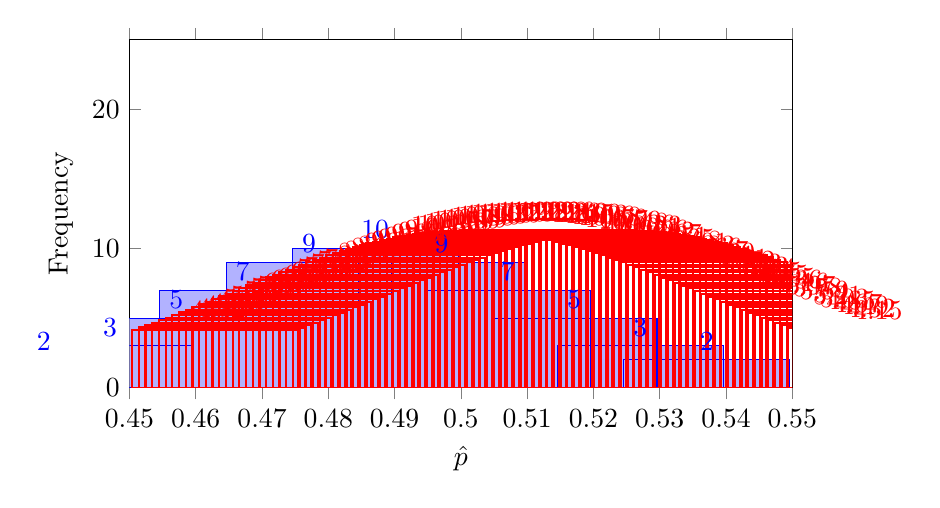
\begin{tikzpicture}
            % Define Gaussian function
            \pgfmathdeclarefunction{gauss}{2}{%
                \pgfmathparse{1/(sqrt(2*pi)*#2)*exp(-((x-#1)^2)/(2*#2^2))}%
            }
            \begin{axis}[
                ybar,
                xmin=0.45, xmax=0.55,
                xtick={0.45,0.46,0.47,0.48,0.49,0.50,0.51,0.52,0.53,0.54,0.55},
                ymin=0, ymax=25,
                ylabel={Frequency},
                xlabel={\( \hat{p} \)},
                width=10cm,
                height=6cm,
                bar width=0.025, % Adjusted for better fit
                nodes near coords,
                nodes near coords align={vertical},
            ]
                \addplot coordinates {
                    (0.45,2) (0.46,3) (0.47,5) (0.48,7) (0.49,9)
                    (0.50,10) (0.51,9) (0.52,7) (0.53,5) (0.54,3)
                    (0.55,2)
                };
                % Overlay Gaussian curve
                \addplot [domain=0.45:0.55, samples=100, red, thick] {gauss(0.50, 0.03535)};
            \end{axis}
        \end{tikzpicture}
        \caption{Sampling Distribution of \( \hat{p} \) around \( p = 0.50 \)}
    \end{figure}
\end{frame}

% Slide 10: Review of Sampling Distribution & Standard Error (SE)
\begin{frame}{Review of Sampling Distribution \& Standard Error (SE)}
    \begin{itemize}
        \item \textbf{Sampling Distribution of \( \hat{p} \):}
        \[
            \hat{p} \sim N\left(p, \frac{p(1 - p)}{n}\right)
        \]
        \item \textbf{Standard Error (SE):}
        \[
            SE = \sqrt{\frac{p(1 - p)}{n}}
        \]
        \item \textbf{Example with Mean:}
        \[
            SE_{\bar{x}} = \frac{\sigma}{\sqrt{n}}
        \]
        \[
            \bar{x} \sim N\left(\mu, \frac{\sigma}{\sqrt{n}}\right)
        \]
    \end{itemize}
    \[
        \text{Central Limit Theorem (CLT): For large } n, \quad \hat{p} \approx N\left(p, \frac{p(1 - p)}{n}\right)
    \]
\end{frame}

% Slide 11: Quantifying Uncertainty with Confidence Intervals
\begin{frame}{Quantifying Uncertainty with Confidence Intervals}
    \begin{itemize}
        \item \textbf{Confidence Interval (CI):} Range within which the true population proportion \( p \) lies with a specified probability.
        \item \textbf{Interpretation:}
        \[
            \text{95\% CI: } [\hat{p} - Z_{0.025} \cdot SE, \hat{p} + Z_{0.025} \cdot SE]
        \]
        \[
            P\left(\hat{p} - Z_{\alpha/2} \cdot SE \leq p \leq \hat{p} + Z_{\alpha/2} \cdot SE\right) = 1 - \alpha
        \]
    \end{itemize}
    \[
        \text{CI} = \hat{p} \pm Z_{\alpha/2} \cdot \sqrt{\frac{\hat{p}(1 - \hat{p})}{n}}
    \]
\end{frame}

% Slide 12: Impact of Confidence Interval Width
\begin{frame}{Impact of Confidence Interval Width}
    \begin{itemize}
        \item \textbf{Wide CI:}
        \begin{itemize}
            \item Indicates high uncertainty.
            \item Greater range of plausible values for \( p \).
            \item Associated with higher confidence levels (e.g., 99\%).
        \end{itemize}
        \item \textbf{Narrow CI:}
        \begin{itemize}
            \item Indicates low uncertainty.
            \item Smaller range of plausible values for \( p \).
            \item Associated with lower confidence levels (e.g., 90\%).
        \end{itemize}
    \end{itemize}
    \[
        \text{Width} = 2 \cdot Z_{\alpha/2} \cdot SE
    \]
    \[
        \text{Higher } Z_{\alpha/2} \Rightarrow \text{Wider CI}
    \]
    \[
        \text{Smaller } SE \Rightarrow \text{Narrower CI}
    \]
    \[
        \text{Law of Large Numbers: } \hat{p} \to p \text{ as } n \to \infty
    \]
\end{frame}

% Slide 13: The Role of Sample Size (n)
\begin{frame}{The Role of Sample Size (\( n \))}
    \begin{itemize}
        \item \textbf{Larger \( n \):}
        \begin{itemize}
            \item Decreases \( SE \).
            \item Narrows the CI.
            \item Increases precision of \( \hat{p} \).
        \end{itemize}
        \item \textbf{Smaller \( n \):}
        \begin{itemize}
            \item Increases \( SE \).
            \item Widens the CI.
            \item Decreases precision of \( \hat{p} \).
        \end{itemize}
    \end{itemize}
    \[
        SE = \sqrt{\frac{p(1 - p)}{n}} \quad \Rightarrow \quad SE \propto \frac{1}{\sqrt{n}}
    \]
    \[
        \text{As } n \uparrow, \quad SE \downarrow \quad \text{and thus} \quad \text{Width} \downarrow
    \]
    \[
        \text{Law of Large Numbers: } \hat{p} \to p \text{ as } n \to \infty
    \]
\end{frame}

% Slide 14: Assumption of Large Sample Size
\begin{frame}{Assumption of Large Sample Size}
    \begin{itemize}
        \item \textbf{Focus for This Lecture:}
        \begin{itemize}
            \item Assume a large sample size (\( n \) is large).
            \item Enables the use of the normal approximation for the sampling distribution of \( \hat{p} \).
        \end{itemize}
        \item \textbf{Mathematical Condition:}
        \[
            np \geq 10 \quad \text{and} \quad n(1 - p) \geq 10
        \]
        \item \textbf{Importance:}
        \begin{itemize}
            \item Validates the Central Limit Theorem (CLT) applicability.
        \end{itemize}
        \item \textbf{Note for Future Lectures:}
        \begin{itemize}
            \item For small sample sizes, exact methods or alternative distributions are required.
            \item Specific population distribution assumptions (e.g., binomial) must be considered.
        \end{itemize}
    \end{itemize}
\end{frame}

% Slide 15: Formal Derivation: Binomial to Normal Approximation
\begin{frame}{From Binomial to Normal: Formal Derivation}
    \begin{itemize}
        \item \textbf{Binary Outcomes:} Each trial results in success (1) or failure (0).
        \item \textbf{Binomial Distribution:}
        \[
            X \sim \text{Binomial}(n, p)
        \]
        \item \textbf{Proportion Calculation:}
        \[
            \hat{p} = \frac{X}{n}
        \]
        \item \textbf{Mean and Variance of \( \hat{p} \):}
        \[
            E(\hat{p}) = p
        \]
        \[
            \text{Var}(\hat{p}) = \frac{p(1 - p)}{n}
        \]
        \item \textbf{Central Limit Theorem Application:}
        \[
            X \approx N(np, np(1 - p)) \quad \text{for large } n
        \]
        \[
            \hat{p} \approx N\left(p, \frac{p(1 - p)}{n}\right)
        \]
        \item \textbf{Standardizing \( \hat{p} \):}
        \[
            Z = \frac{\hat{p} - p}{\sqrt{\frac{p(1 - p)}{n}}} \sim N(0, 1)
        \]
    \end{itemize}
\end{frame}

% Slide 16: Derivation of the Confidence Interval Formula
\begin{frame}{Derivation of the Confidence Interval Formula}
    \begin{itemize}
        \item \textbf{Starting Point:}
        \[
            \hat{p} \approx N\left(p, \frac{p(1 - p)}{n}\right)
        \]
        \item \textbf{Standardizing \( \hat{p} \):}
        \[
            Z = \frac{\hat{p} - p}{\sqrt{\frac{p(1 - p)}{n}}} \sim N(0, 1)
        \]
        \item \textbf{Constructing the Confidence Interval:}
        \[
            P\left(-Z_{\alpha/2} \leq Z \leq Z_{\alpha/2}\right) = 1 - \alpha
        \]
        \[
            P\left(-Z_{\alpha/2} \leq \frac{\hat{p} - p}{\sqrt{\frac{p(1 - p)}{n}}} \leq Z_{\alpha/2}\right) = 1 - \alpha
        \]
        \item \textbf{Solving for \( p \):}
        \[
            -Z_{\alpha/2} \sqrt{\frac{p(1 - p)}{n}} \leq \hat{p} - p \leq Z_{\alpha/2} \sqrt{\frac{p(1 - p)}{n}}
        \]
        \[
            \hat{p} - Z_{\alpha/2} \sqrt{\frac{p(1 - p)}{n}} \leq p \leq \hat{p} + Z_{\alpha/2} \sqrt{\frac{p(1 - p)}{n}}
        \]
        \item \textbf{Confidence Interval for \( p \):}
        \[
            p \in \left[ \hat{p} - Z_{\alpha/2} \sqrt{\frac{\hat{p}(1 - \hat{p})}{n}}, \hat{p} + Z_{\alpha/2} \sqrt{\frac{\hat{p}(1 - \hat{p})}{n}} \right]
        \]
        \[
            \text{Note: Substitute } p \text{ with } \hat{p} \text{ in the standard error as } p \text{ is unknown.}
        \]
    \end{itemize}
    \[
        \text{Confidence Interval (CI)} = \hat{p} \pm Z_{\alpha/2} \cdot \sqrt{\frac{\hat{p}(1 - \hat{p})}{n}}
    \]
\end{frame}

% Slide 17: Confidence Intervals for Proportions
\begin{frame}{Confidence Intervals for Proportions}
    \begin{itemize}
        \item \textbf{Formula:}
        \[
            \text{CI} = \hat{p} \pm Z_{\alpha/2} \cdot \sqrt{\frac{\hat{p}(1 - \hat{p})}{n}}
        \]
        \item \textbf{Components:}
        \begin{itemize}
            \item \( \hat{p} \): Sample proportion
            \item \( Z_{\alpha/2} \): Critical value from the standard normal distribution
            \item \( \sqrt{\frac{\hat{p}(1 - \hat{p})}{n}} \): Standard error of \( \hat{p} \)
        \end{itemize}
        \item \textbf{Critical Value Selection:}
        \begin{itemize}
            \item 95\% CI: \( Z_{0.025} = 1.96 \)
            \item 99\% CI: \( Z_{0.005} = 2.576 \)
        \end{itemize}
    \end{itemize}
\end{frame}

% Slide 18: Choosing a Confidence Level
\begin{frame}{Choosing a Confidence Level}
    \begin{itemize}
        \item \textbf{Common Confidence Levels:}
        \begin{itemize}
            \item 90\% (\( Z_{0.05} = 1.645 \))
            \item 95\% (\( Z_{0.025} = 1.96 \))
            \item 99\% (\( Z_{0.005} = 2.576 \))
        \end{itemize}
        \item \textbf{Trade-Off:}
        \begin{itemize}
            \item \textbf{Higher Confidence Level:} Wider CI
            \item \textbf{Lower Confidence Level:} Narrower CI
        \end{itemize}
        \item \textbf{Mathematical Representation:}
        \[
            \text{CI} = \hat{p} \pm Z_{\alpha/2} \cdot \sqrt{\frac{\hat{p}(1 - \hat{p})}{n}}
        \]
    \end{itemize}
\end{frame}

% Slide 19: Example: Calculating a Confidence Interval
\begin{frame}{Example: Calculating a Confidence Interval}
    \textbf{Problem Statement:}
    \begin{itemize}
        \item \(\hat{p} = 0.60\) (60\% vaccinated)
        \item \(n = 200\) (sample size)
        \item \textbf{Confidence Level:} 95\%
    \end{itemize}

    \textbf{Mathematical Steps:}
    \begin{enumerate}
        \item \textbf{Calculate Standard Error (SE):}
        \[
            SE = \sqrt{\frac{\hat{p}(1 - \hat{p})}{n}} = \sqrt{\frac{0.60 \times 0.40}{200}} = \sqrt{\frac{0.24}{200}} = \sqrt{0.0012} \approx 0.0346
        \]
        \item \textbf{Find Critical Value (\( Z_{\alpha/2} \)):}
        \[
            Z_{0.025} = 1.96 \quad \text{for 95\% CI}
        \]
        \item \textbf{Compute Margin of Error (ME):}
        \[
            ME = Z_{\alpha/2} \times SE = 1.96 \times 0.0346 \approx 0.0678
        \]
        \item \textbf{Determine Confidence Interval (CI):}
        \[
            \text{CI} = \hat{p} \pm ME = 0.60 \pm 0.0678 = [0.5322, 0.6678]
        \]
        \[
            \text{Rounded: } [0.533, 0.668]
        \]
    \end{enumerate}

    \textbf{Conclusion:}
    \[
        \text{We are 95\% confident that the true proportion of vaccinated individuals is between } 53.3\% \text{ and } 66.8\%.
    \]
\end{frame}

% Slide 20: Visual for Example: Calculating a Confidence Interval
\begin{frame}{Visualizing Confidence Interval Calculation}
    \begin{figure}
        \centering
        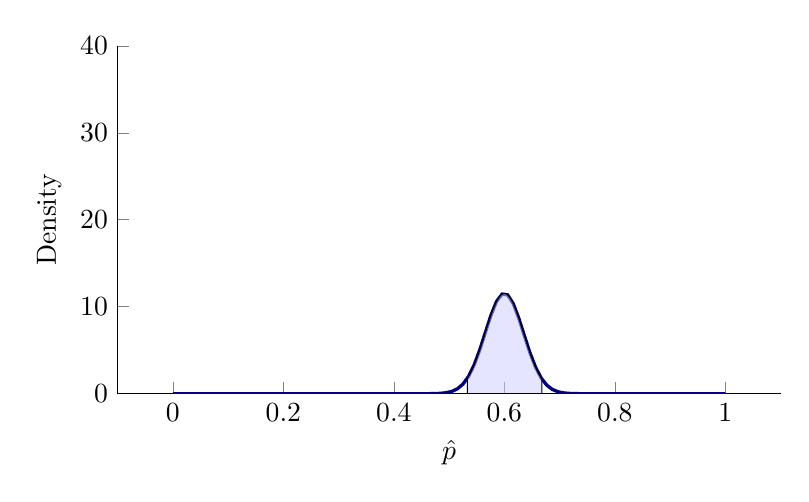
\begin{tikzpicture}
            % Define Gaussian function
            \pgfmathdeclarefunction{gauss}{2}{%
                \pgfmathparse{1/(sqrt(2*pi)*#2)*exp(-((x-#1)^2)/(2*#2^2))}%
            }
            \begin{axis}[
                no markers, domain=0:1, samples=100,
                axis lines*=left,
                xlabel={\( \hat{p} \)},
                ylabel={Density},
                height=6cm, width=10cm,
                ymin=0, ymax=40,
            ]
                % Plot the normal distribution centered at p=0.60 with SE=0.0346
                \addplot [very thick, blue!50!black] {gauss(0.60, 0.0346)};
                % Shade the confidence interval area
                \addplot [
                    domain=0.533:0.668,
                    samples=100,
                    fill=blue!20,
                    fill opacity=0.5
                ] {gauss(0.60, 0.0346)} \closedcycle;
            \end{axis}
        \end{tikzpicture}
        \caption{Confidence Interval Visualization}
    \end{figure}
\end{frame}

% Slide 21: Interpretation of the Confidence Interval
\begin{frame}{Interpretation of the Confidence Interval}
    \begin{itemize}
        \item \textbf{Explanation:}
        \[
            \text{We are 95\% confident that the true population proportion } p \text{ lies between } 53.3\% \text{ and } 66.8\%.
        \]
        \item \textbf{Implications:}
        \begin{itemize}
            \item \textbf{Narrow Interval:} Indicates high precision in the estimate.
            \item \textbf{Wide Interval:} Indicates low precision, possibly due to smaller sample size or higher variability.
        \end{itemize}
    \end{itemize}
    \[
        0.533 \leq p \leq 0.668 \quad \text{with 95\% confidence}
    \]
\end{frame}

% Slide 22: Introducing Hypothesis Testing for Proportions
\begin{frame}{Introducing Hypothesis Testing for Proportions}
    \begin{itemize}
        \item \textbf{Objective:} Assess whether the observed sample proportion \( \hat{p} \) provides sufficient evidence to infer that the population proportion \( p \) differs from a specified value \( p_0 \).
        \item \textbf{Components:}
        \begin{itemize}
            \item \textbf{Null Hypothesis (\( H_0 \)):}
            \[
                H_0: p = p_0
            \]
            \item \textbf{Alternative Hypothesis (\( H_a \)):}
            \[
                H_a: p \neq p_0 \quad \text{(Two-tailed)}
            \]
        \end{itemize}
        \item \textbf{Example Context:}
        \[
            H_0: p = 0.50 \quad vs. \quad H_a: p \neq 0.50
        \]
        \[
            \text{(e.g., testing if the vaccination campaign has changed the vaccination rate from 50\%)}
        \]
    \end{itemize}
\end{frame}

% Slide 23: Test Statistic for Proportion
\begin{frame}{Test Statistic for Proportion}
    \begin{itemize}
        \item \textbf{Formula:}
        \[
            Z = \frac{\hat{p} - p_0}{\sqrt{\frac{p_0(1 - p_0)}{n}}}
        \]
        \item \textbf{Components:}
        \begin{itemize}
            \item \( \hat{p} \): Sample proportion
            \item \( p_0 \): Hypothesized population proportion
            \item \( n \): Sample size
        \end{itemize}
        \item \textbf{Interpretation:}
        \[
            Z \text{ measures how many standard errors } \hat{p} \text{ is away from } p_0.
        \]
    \end{itemize}
    \[
        Z \sim N(0,1) \quad \text{under } H_0
    \]
\end{frame}

% Slide 24: P-Value and Decision Rule
\begin{frame}{P-Value and Decision Rule}
    \begin{itemize}
        \item \textbf{P-Value Definition:}
        \[
            \text{The probability of observing a test statistic as extreme as, or more extreme than, the observed } Z \text{ under } H_0.
        \]
        \item \textbf{Decision Rule:}
        \[
            \text{If } p\text{-value} < \alpha, \text{ reject } H_0
        \]
        \item \textbf{Common Significance Level (\( \alpha \)):} 0.05
        \item \textbf{Mathematical Insight:}
        \[
            \text{Two-Tailed Test: } p\text{-value} = 2 \times P(Z > |Z_{\text{obs}}|)
        \]
    \end{itemize}
\end{frame}

% Slide 25: Example: Hypothesis Test for Proportion
\begin{frame}{Example: Hypothesis Test for Proportion}
    \textbf{Problem Statement:}
    \begin{itemize}
        \item \(\hat{p} = 0.60\) (60\% vaccinated)
        \item \(n = 200\) (sample size)
        \item \textbf{Hypotheses:}
        \[
            H_0: p = 0.50 \quad vs. \quad H_a: p \neq 0.50
        \]
    \end{itemize}

    \textbf{Mathematical Steps:}
    \begin{enumerate}
        \item \textbf{Compute the Test Statistic (\( Z \)):}
        \[
            Z = \frac{\hat{p} - p_0}{\sqrt{\frac{p_0(1 - p_0)}{n}}} = \frac{0.60 - 0.50}{\sqrt{\frac{0.50 \times 0.50}{200}}} = \frac{0.10}{\sqrt{0.00125}} = \frac{0.10}{0.03535} \approx 2.828
        \]
        \item \textbf{Determine the P-Value:}
        \[
            P(Z > 2.828) \approx 0.0023
        \]
        \[
            \text{Since it's a two-tailed test: } p\text{-value} = 2 \times 0.0023 = 0.0046
        \]
        \item \textbf{Decision:}
        \[
            0.0046 < 0.05 \Rightarrow \text{Reject } H_0
        \]
    \end{enumerate}

    \textbf{Conclusion:}
    \[
        \text{There is significant evidence to reject } H_0. \text{ The true vaccination rate } p \text{ is different from } 0.50.
    \]
\end{frame}

% Slide 26: Visual for Example: Hypothesis Test for Proportion
\begin{frame}{Visualizing Hypothesis Test Calculation}
    \begin{figure}
        \centering
        \begin{tikzpicture}
            % Define Gaussian function
            \pgfmathdeclarefunction{gauss}{2}{%
                \pgfmathparse{1/(sqrt(2*pi)*#2)*exp(-((x-#1)^2)/(2*#2^2))}%
            }
            \begin{axis}[
                no markers, domain=0:1, samples=100,
                axis lines*=left,
                xlabel={\( \hat{p} \)},
                ylabel={Density},
                height=6cm, width=10cm,
                ymin=0, ymax=40,
            ]
                % Plot the null hypothesis distribution centered at p0=0.50 with SE=0.03535
                \addplot [very thick, blue!50!black] {gauss(0.50, 0.03535)};
                % Shade the rejection regions
                \addplot [
                    domain=0.50 + 1.96*0.03535:1,
                    samples=100,
                    fill=red!30,
                    fill opacity=0.5
                ] {gauss(0.50, 0.03535)} \closedcycle;

                \addplot [
                    domain=0:0.50 - 1.96*0.03535,
                    samples=100,
                    fill=red!30,
                    fill opacity=0.5
                ] {gauss(0.50, 0.03535)} \closedcycle;

                % Mark the observed sample proportion p=0.60
                \draw[thick, dashed, green!60!black] (axis cs:0.60,0) -- (axis cs:0.60, {gauss(0.50, 0.03535)});
                \node[above] at (axis cs:0.60, {gauss(0.50, 0.03535)}) {\footnotesize \( \hat{p} = 0.60 \)};

                % Label p0=0.50
                \draw[thick, dashed, blue!50!black] (axis cs:0.50,0) -- (axis cs:0.50, {gauss(0.50, 0.03535)});
                \node[below] at (axis cs:0.50,0) {\footnotesize \( p_0 = 0.50 \)};
            \end{axis}
        \end{tikzpicture}
        \caption{Hypothesis Test Visualization}
    \end{figure}
\end{frame}

% Slide 27: Interpretation of Hypothesis Test Result
\begin{frame}{Interpretation of Hypothesis Test Result}
    \begin{itemize}
        \item \textbf{Conclusion:}
        \[
            \text{Significant evidence to reject } H_0.
        \]
        \[
            \text{The true vaccination rate } p \text{ is different from } 0.50.
        \]
        \item \textbf{Implications:}
        \begin{itemize}
            \item \textbf{Public Health Decision:} The vaccination campaign has significantly altered vaccination rates.
            \item \textbf{Policy Adjustment:} Potentially scaling up or modifying the campaign based on results.
        \end{itemize}
    \end{itemize}
    \[
        p \neq 0.50 \quad \text{with } p\text{-value} = 0.0046
    \]
\end{frame}

% Slide 28: Comparing Confidence Intervals and Hypothesis Testing
\begin{frame}{Comparing Confidence Intervals and Hypothesis Testing}
    \begin{itemize}
        \item \textbf{Connection:}
        \[
            H_0: p = p_0 \quad \text{is rejected} \iff p_0 \notin \text{CI}
        \]
        \item \textbf{Implication:}
        \[
            \text{Consistent conclusions from both Confidence Intervals and Hypothesis Testing methods.}
        \]
    \end{itemize}
    \[
        p_0 \notin [\hat{p} - Z_{\alpha/2} \cdot SE, \hat{p} + Z_{\alpha/2} \cdot SE] \Rightarrow \text{Reject } H_0
    \]
\end{frame}

% Slide 29: Visual for Comparing CI & Hypothesis Testing
\begin{frame}{Visual Comparison of CI \& Hypothesis Testing}
    \begin{figure}
        \centering
        \begin{tikzpicture}
            % Define Gaussian function
            \pgfmathdeclarefunction{gauss}{2}{%
                \pgfmathparse{1/(sqrt(2*pi)*#2)*exp(-((x-#1)^2)/(2*#2^2))}%
            }
            \begin{axis}[
                no markers, domain=0:1, samples=100,
                axis lines*=left,
                xlabel={\( \hat{p} \)},
                ylabel={Density},
                height=6cm, width=10cm,
                ymin=0, ymax=40,
            ]
                % Plot the confidence interval distribution centered at p=0.60 with SE=0.0346
                \addplot [very thick, blue!50!black] {gauss(0.60, 0.0346)};
                % Shade the confidence interval area
                \addplot [
                    domain=0.533:0.668,
                    samples=100,
                    fill=blue!20,
                    fill opacity=0.5
                ] {gauss(0.60, 0.0346)} \closedcycle;

                % Mark p0=0.50 outside the CI
                \draw[thick, dashed, red!50!black] (axis cs:0.50,0) -- (axis cs:0.50, {gauss(0.60, 0.0346)});
                \node[below] at (axis cs:0.50,0) {\footnotesize \( p_0 = 0.50 \)};
            \end{axis}
        \end{tikzpicture}
        \caption{CI and Hypothesis Test Comparison}
    \end{figure}
\end{frame}



% Slide 30: Guided Practice Activity
\begin{frame}{Guided Practice Activity}
    \begin{itemize}
        \item \textbf{Task:}
        \begin{itemize}
            \item Calculate Confidence Interval (CI) and perform Hypothesis Test for given \( \hat{p} \) and \( n \).
        \end{itemize}
        \item \textbf{Example Scenario:}
        \[
            \text{Proportion of people vaccinated in a different public health initiative.}
        \]
        \item \textbf{Sample Data:}
        \[
            \hat{p} = 0.55, \quad n = 300, \quad H_0: p = 0.50
        \]
        \item \textbf{Instructions:}
        \begin{enumerate}
            \item Calculate Standard Error (SE):
            \[
                SE = \sqrt{\frac{\hat{p}(1 - \hat{p})}{n}} = \sqrt{\frac{0.55 \times 0.45}{300}} \approx \sqrt{\frac{0.2475}{300}} \approx \sqrt{0.000825} \approx 0.0287
            \]
            \item Compute Confidence Interval (CI):
            \[
                \text{CI} = 0.55 \pm 1.96 \times SE = 0.55 \pm 1.96 \times 0.0287 \approx 0.55 \pm 0.0563 = [0.4937, 0.6063]
            \]
            \[
                \text{Rounded: } [0.494, 0.606]
            \]
            \item Perform Hypothesis Test:
            \begin{enumerate}
                \item Calculate \( Z \)-score:
                \[
                    Z = \frac{\hat{p} - p_0}{\sqrt{\frac{p_0(1 - p_0)}{n}}} = \frac{0.55 - 0.50}{\sqrt{\frac{0.50 \times 0.50}{300}}} = \frac{0.05}{\sqrt{0.000833}} \approx \frac{0.05}{0.0289} \approx 1.73
                \]
                \item Determine \( p\text{-value} \):
                \[
                    P(Z > 1.73) \approx 0.0418
                \]
                \[
                    \text{Since it's a two-tailed test: } p\text{-value} = 2 \times 0.0418 = 0.0836
                \]
                \item Make a decision based on \( \alpha = 0.05 \):
                \[
                    0.0836 > 0.05 \Rightarrow \text{Fail to Reject } H_0
                \]
            \end{enumerate}
        \end{enumerate}
    \end{itemize}
\end{frame}

% Slide 31: Practice Problem Walkthrough
\begin{frame}{Practice Problem Walkthrough}
    \textbf{Example Problem:}
    \begin{itemize}
        \item \(\hat{p} = 0.45\)
        \item \(n = 150\)
        \item \textbf{Confidence Level:} 95\%
        \item \textbf{Hypotheses:}
        \[
            H_0: p = 0.40 \quad vs. \quad H_a: p \neq 0.40
        \]
    \end{itemize}

    \textbf{Mathematical Steps:}
    \begin{enumerate}
        \item \textbf{Calculate Standard Error (SE):}
        \[
            SE = \sqrt{\frac{\hat{p}(1 - \hat{p})}{n}} = \sqrt{\frac{0.45 \times 0.55}{150}} = \sqrt{\frac{0.2475}{150}} = \sqrt{0.00165} \approx 0.0406
        \]
        \item \textbf{Compute Confidence Interval (CI):}
        \[
            ME = Z_{0.025} \times SE = 1.96 \times 0.0406 \approx 0.0796
        \]
        \[
            \text{CI} = 0.45 \pm 0.0796 = [0.3704, 0.5296] \quad \text{(Rounded: [0.370, 0.530])}
        \]
        \item \textbf{Perform Hypothesis Test:}
        \begin{enumerate}
            \item \textbf{Calculate \( Z \)-Statistic:}
            \[
                Z = \frac{0.45 - 0.40}{\sqrt{\frac{0.40 \times 0.60}{150}}} = \frac{0.05}{\sqrt{\frac{0.24}{150}}} = \frac{0.05}{0.0400} = 1.25
            \]
            \item \textbf{Determine P-Value:}
            \[
                P(Z > 1.25) \approx 0.1056
            \]
            \[
                \text{Since it's a two-tailed test: } p\text{-value} = 2 \times 0.1056 = 0.2112
            \]
            \item \textbf{Decision:}
            \[
                0.2112 > 0.05 \Rightarrow \text{Fail to Reject } H_0
            \]
        \end{enumerate}
    \end{enumerate}

    \textbf{Conclusion:}
    \[
        \text{Fail to reject } H_0. \text{ There is insufficient evidence to conclude that } p \neq 0.40.
    \]

    \textbf{Mathematical Alignment:}
    \[
        p_0 = 0.40 \in \text{CI} = [0.370, 0.530] \Rightarrow \text{Do not reject } H_0
    \]
\end{frame}

% Slide 32: Summary & Key Takeaways
\begin{frame}{Summary \& Key Takeaways}
    \begin{itemize}
        \item \textbf{Confidence Intervals:}
        \begin{itemize}
            \item Quantify uncertainty around \( \hat{p} \).
            \item Depend on sample size (\( n \)) and variability (\( \hat{p}(1 - \hat{p}) \)).
            \item Formula:
            \[
                \text{CI} = \hat{p} \pm Z_{\alpha/2} \cdot \sqrt{\frac{\hat{p}(1 - \hat{p})}{n}}
            \]
        \end{itemize}
        \item \textbf{Hypothesis Testing:}
        \begin{itemize}
            \item Evaluate assumptions about \( p \).
            \item Utilize \( Z \)-test for proportions.
            \item Decision based on \( p\text{-value} \) and significance level (\( \alpha \)).
            \item Formula for \( Z \)-score:
            \[
                Z = \frac{\hat{p} - p_0}{\sqrt{\frac{p_0(1 - p_0)}{n}}}
            \]
        \end{itemize}
        \item \textbf{Sample Size (\( n \)):}
        \begin{itemize}
            \item Larger \( n \) decreases \( SE \), leading to narrower CIs and more powerful tests.
        \end{itemize}
        \item \textbf{Relationship Between CI and Hypothesis Testing:}
        \begin{itemize}
            \item Consistency in conclusions: If \( p_0 \) lies outside the CI, \( H_0 \) is rejected.
        \end{itemize}
    \end{itemize}
    \[
        \text{CI: } \hat{p} \pm Z_{\alpha/2} \cdot \sqrt{\frac{\hat{p}(1 - \hat{p})}{n}}
    \]
    \[
        Z = \frac{\hat{p} - p_0}{\sqrt{\frac{p_0(1 - p_0)}{n}}}
    \]
\end{frame}

\end{document}


The procedure for computing a confidence interval is a
Set-valued correspondence.

So is a random set-valued correspondence.

Sweet — let’s dive a bit deeper now into the statistical and mathematical framing of this idea. You’re basically sitting at the intersection of **statistics** and **functional analysis/econ theory**, where set-valued mappings come up a lot.

---

### �� Framing in **Statistics**
In statistics, especially in estimation theory and decision theory:

- A confidence interval procedure can be seen as a **mapping** from data (or a summary like \( (n, \hat{p}) \)) to a **subset of the parameter space** (here, the interval in \([0,1]\) for a proportion).

This mapping is **not random** once \( (n, \hat{p}) \) is fixed — it deterministically gives you an interval. So:

> It **is** a function — but a function that returns a **set**, not a scalar. Hence, it’s a **set-valued function**.

---

### �� In **Math (Topology/Econ/Functional Analysis)**

Here’s where the language gets sharper. Let’s say you have:

\[
F: X \rightrightarrows Y
\]

This is a **correspondence** (aka **set-valued mapping**) if:
- \( F(x) \subseteq Y \) for each \( x \in X \)
- \( F(x) \) might be a set of possible outcomes — doesn’t have to be single-valued

And we ask questions like:
- Is \( F \) **upper hemicontinuous**? (small changes in input don't explode output)
- Is \( F \) **measurable**? (important for probabilistic/stochastic analysis)
- Does \( F \) have **closed** or **convex** values?

These properties matter a lot in areas like:
- **Game theory** (best response correspondences)
- **Economics** (preference and choice correspondences)
- **Stochastic control** (randomized policies)

---

### ✨ Example in Your Case:

Let’s define the mapping:

\[
F(n, \hat{p}) = \left[\hat{p} - z_{\alpha/2} \sqrt{\frac{\hat{p}(1 - \hat{p})}{n}},\ \hat{p} + z_{\alpha/2} \sqrt{\frac{\hat{p}(1 - \hat{p})}{n}}\right]
\]

Then \( F \) is a **set-valued function** from \( \mathbb{N} \times [0,1] \) to \( \mathcal{P}([0,1]) \) (the power set of [0,1]).

It’s single-valued in the sense that you get a unique interval — but it’s still a **function into sets**, not numbers.

---

### TL;DR

What you’re describing is technically a:

> �� **Set-valued function**
> �� aka **Correspondence** (in math/econ language)

Let me know if you want a visual or want to tie this into measurable correspondences or something more abstract!
